% Progress report -- Adaptive Task Allocation for Heterogeneous Bio-Inspired Agents
% Compiles on Overleaf with the default pdfLaTeX compiler. Single file, no .bib needed.

\documentclass[11pt,a4paper]{article}

\usepackage[T1]{fontenc}
\usepackage{newtxtext,newtxmath}
\usepackage[a4paper,margin=1in]{geometry}
\usepackage{microtype}
\usepackage{parskip}
\usepackage{booktabs,tabularx,array}
\usepackage{enumitem}
\usepackage{titlesec}
\usepackage[font=small,labelfont=bf,labelsep=period]{caption}
\usepackage{xcolor}
\usepackage{tikz}
\usetikzlibrary{positioning,arrows.meta,fit}
\usepackage{placeins}
\usepackage{float}
\usepackage{amsmath}
\usepackage[hidelinks]{hyperref}

\titleformat{\section}{\normalfont\large\bfseries}{\thesection}{0.7em}{}
\titleformat{\subsection}{\normalfont\normalsize\bfseries}{\thesubsection}{0.6em}{}
\titlespacing*{\section}{0pt}{16pt}{4pt}
\titlespacing*{\subsection}{0pt}{10pt}{2pt}
\setlist{itemsep=2pt,topsep=3pt,leftmargin=1.5em}
\renewcommand{\arraystretch}{1.18}
\newcolumntype{L}{>{\raggedright\arraybackslash}X}
\newcolumntype{P}[1]{>{\raggedright\arraybackslash}p{#1}}
\newcommand{\head}[1]{\textbf{#1}}
\newcommand{\runin}[1]{\textbf{#1}\quad}
% Marks a number that the running experiments will fill in. Remove before submission.
\newcommand{\pending}[1]{\textcolor{red!70!black}{[#1]}}
\hyphenation{meta-heu-ris-tic pher-o-mone}
\emergencystretch=1.2em

\begin{document}

\begin{center}
  {\LARGE\bfseries Adaptive Task Allocation for\\[3pt]
  Heterogeneous Bio-Inspired Agents\par}
  \vspace{12pt}
  {\large Phase 1 Progress Report\par}
  \vspace{5pt}
  Final Year B.Tech Project, 2026--27\\
  Department of Computer Science and Engineering\\
  Delhi Technological University\par
  \vspace{8pt}
  {\small Group GP105 (Group Key A4) \quad Guide: Prof.~Shailender Kumar \quad Coordinator: Dr.~Yeshwant Singh}\\[2pt]
  {\small Nikshay Yadav (23/CS/284) \quad Madan Raj Murugesan (23/CS/234) \quad Aryan Varshney (24/CS/111)}\\[2pt]
  {\small 17 November 2026}
\end{center}

\begin{abstract}
\noindent
Multi-agent systems built on large language models (LLMs) usually apply one coordination pattern to every
part of a task, and controlled studies report that they often fail to beat a well-prompted single agent.
This project asks whether a coordinator that chooses a different coordination mechanism for each subtask
can do better within the same token budget. The mechanisms come from animal behaviour and are written as
ordinary algorithms: reinforced search (ant), evidence accumulation with cross inhibition (bee) and bounded
local execution (octopus), each paired with plain controls that lack its distinguishing parts. This report
covers Phase~1. We built \texttt{bioalloc}, a Python framework with a common executor interface, a budget
ledger that admits a model call only if it fits, append-only traces of every call, runtime checks kept
separate from the grader, frozen task splits and a resumable experiment runner. With Claude Sonnet~4.6 as the
backbone we ran smoke tests, a difficulty calibration, a comparison of five systems on PlanBench Logistics
at a 21,000-token cap, a tuning run of redesigned mechanisms on a generated Logistics suite and
\pending{a held-out test}. The single agent solved every calibration task when given a generous budget and
remained the strongest system on Logistics (73\% of runs against 67\% for octopus, 60\% for bee, 57\% for a
single direct call and 0\% for the step-per-call ant). Trace analysis shows why: the single agent revises
its plan against the simulator's message, and the first versions of the mechanisms did not use that
feedback. Choosing the best system per task would have solved 25 of 30 runs instead of 22, which is the room
an allocation policy can use in Phase~2.
\end{abstract}

\section{Introduction}

An LLM multi-agent system splits a task among agents that exchange messages. The split is useful only if
the way the agents coordinate suits the work. A subtask with many possible solution paths may benefit from
exploration that remembers what worked, a subtask with a few competing answers needs those answers compared,
and a well-specified subtask needs no discussion at all. Most current systems choose one pattern for the
whole task. Kim et al.~\cite{kim2025scaling} compared a single agent with four multi-agent architectures
under standardized tools, prompts and compute and found changes from $+80.8\%$ to $-70.0\%$ depending on the
task, and Cemri et al.~\cite{cemri2025mast} traced many failures of popular frameworks to system design and
coordination rather than to the model.

This project studies \emph{adaptive allocation}: a coordinator that, for each subtask of a task graph,
chooses one mechanism from a pool, or answers it with a single direct call, so as to maximize the chance of
a correct final answer within a fixed budget. The pool is bio-inspired, but every mechanism is specified by
what it computes and tested against plain counterparts, following the criticism of metaphor-driven
algorithms by Camacho-Villal\'on et al.~\cite{camacho2023}.

The five research questions of the approved synopsis are: \textbf{RQ1} do the mechanisms have complementary
strengths; \textbf{RQ2} can dynamic allocation improve performance within a fixed budget; \textbf{RQ3} what
value do the biological mechanisms add over conventional ones; \textbf{RQ4} can the framework adapt to
failures; and \textbf{RQ5} when does coordination stop paying for itself.

\runin{Phase 1 contributions.}
\begin{enumerate}[label=(\arabic*)]
  \item A framework in which mechanisms, baselines and controls share one model, one solving prompt, one
        stored decomposition, the same checks and an equal, enforced token budget (Section~\ref{sec:system}).
  \item Ant, bee and octopus executors with their controls; single-agent, direct, majority-vote,
        plan-then-execute and specialist baselines; rule-table and LinUCB~\cite{li2010linucb} policies.
  \item Task suites with automatic checking: GSM8K~\cite{cobbe2021gsm8k}, PlanBench~\cite{valmeekam2023planbench}
        with our own plan simulator, a deterministic tool suite, a controlled synthetic suite, and 180
        generated Logistics problems, all in frozen, hashed splits.
  \item A measured first answer to parts of RQ1, RQ3 and RQ5 on long-horizon planning, an explanation of
        the results from the traces, and redesigned mechanisms that use feedback
        (Section~\ref{sec:results}).
\end{enumerate}

\section{Related Work}
\label{sec:lit}

\runin{Fixed workflows and their cost.}
He, Treude and Lo~\cite{he2025lma} review 71 studies of LLM multi-agent systems in software engineering
and name the optimization of agent collaboration as an open phase of research. Cemri et
al.~\cite{cemri2025mast} built a taxonomy of 14 failure modes from 150 traces and used it to annotate more
than 1,600 traces of seven frameworks. Wang et al.~\cite{wang2024rethinking} found that a single agent with a
strong prompt comes close to the best multi-agent discussion method on reasoning benchmarks, and Zhang et
al.~\cite{zhang2025agentprune} showed that many inter-agent messages can be pruned.

\runin{Adaptive topology and routing.}
GPTSwarm~\cite{zhuge2024gptswarm} optimizes agent graphs, DyLAN~\cite{liu2024dylan} selects teams,
G-Designer~\cite{zhang2025gdesigner} generates a topology per task, AFlow~\cite{zhang2025aflow} searches
workflows written as code, and RouteLLM~\cite{ong2025routellm} routes queries between models.
MasRouter~\cite{yue2025masrouter} chooses the collaboration mode, roles and models together.
GraphPlanner~\cite{feng2026graphplanner}, AdaptOrch~\cite{yu2026adaptorch} and
Symphony-Coord~\cite{guan2026symphony} route at the level of steps or subtasks; the last uses a LinUCB bandit
over task and agent features, as our learned policy will. In all of them the candidates are agents, roles,
models or graph shapes, not coordination mechanisms with their own control flow.

\runin{Bio-inspired coordination with LLMs.}
Wu et al.~\cite{wu2025ecllm} survey LLMs and evolutionary computation. AMRO-S~\cite{wang2026amros} and
SwarmSys~\cite{li2025swarmsys} apply ant-colony rules to routing and task allocation. Rahman et
al.~\cite{rahman2026swarms} found that an LLM version of Boids needed about 300 times the computation of the
classical one, a warning we take seriously by holding compute equal. The mechanisms we implement come from
ant colony optimization~\cite{dorigo2004aco}, honeybee nest-site selection with cross
inhibition~\cite{seeley2012} (whose nearest software relative is self-consistency voting~\cite{wang2023selfconsistency})
and the peripheral motor programs of the octopus arm~\cite{sumbre2001}.

\runin{Gap.}
No prior system chooses between whole coordination mechanisms per subtask and tests each one against
controls without its biological components at equal compute. That is the gap this project addresses.

\section{Problem Formulation}

A task is decomposed into a dependency graph $G=(V,E)$ of subtasks. A pool
$\mathcal{M}=\{m_1,\dots,m_K\}$ of mechanisms is available behind one interface, together with a direct
route that answers a subtask with one model call. For each ready subtask $v$ the coordinator chooses
$\pi(v)\in\mathcal{M}\cup\{\text{direct}\}$ from features observable before execution and from recorded
outcomes. It sees only runtime checks, never reference answers. The aim is
\begin{equation}
  \max_{\pi}\ \Pr[\text{final answer correct}] \quad \text{subject to} \quad
  \mathrm{tokens}(\pi) \le B,
\end{equation}
where the token count includes the coordinator's own calls and any reallocation after a failed check. A
wrong choice is paid twice: once in wasted budget and once in the reallocation that follows.

\section{System Design}
\label{sec:system}

\begin{figure}[H]
\centering
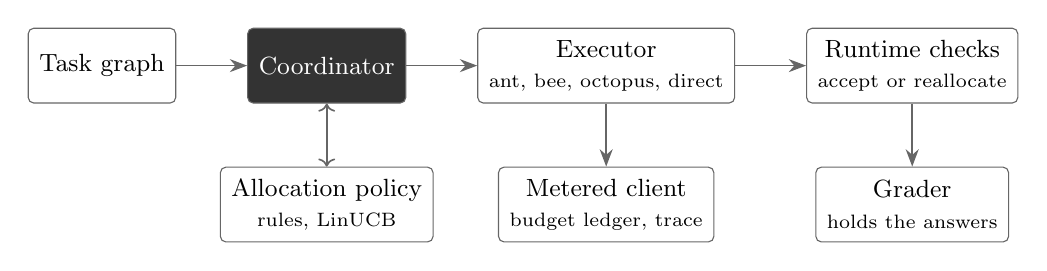
\begin{tikzpicture}[
  box/.style={draw=black!60, rounded corners=2pt, align=center, minimum height=0.95cm, font=\small, inner sep=4pt},
  dark/.style={box, fill=black!80, text=white},
  arr/.style={-{Stealth[length=2.2mm]}, black!60, line width=0.6pt}]
  \node[box] (g) {Task graph};
  \node[dark, right=0.9cm of g] (c) {Coordinator};
  \node[box, below=0.8cm of c] (p) {Allocation policy\\\scriptsize rules, LinUCB};
  \node[box, right=0.9cm of c] (e) {Executor\\\scriptsize ant, bee, octopus, direct};
  \node[box, below=0.8cm of e] (m) {Metered client\\\scriptsize budget ledger, trace};
  \node[box, right=0.9cm of e] (k) {Runtime checks\\\scriptsize accept or reallocate};
  \node[box, below=0.8cm of k] (r) {Grader\\\scriptsize holds the answers};
  \draw[arr] (g) -- (c);
  \draw[arr, <->] (c) -- (p);
  \draw[arr] (c) -- (e);
  \draw[arr] (e) -- (m);
  \draw[arr] (e) -- (k);
  \draw[arr] (k) -- (r);
\end{tikzpicture}
\caption{The \texttt{bioalloc} framework. Only the grader, which lives in the evaluation package, holds
reference answers; nothing outside that package may import it (enforced by a test).}
\label{fig:arch}
\end{figure}

\subsection{Coordinator and executors}
The coordinator repeatedly takes the subtasks whose dependencies are done, asks the policy which executor
should handle each one, dispatches it under a child budget account, checks the result and either accepts it
or reallocates the subtask with the rejection reason. When every final subtask is accepted, a deterministic
family-specific aggregator builds the answer. Executors implement one method,
\texttt{execute(subtask, context)}, and differ only in control flow, communication, memory and stopping. The
context carries accepted upstream outputs, earlier rejections, a metered client, a derived seed and a trace
hook.

\subsection{Budget ledger}
Every model call reserves an estimate of its prompt plus its maximum completion before it is sent. If the
reservation does not fit in what the dispatch and all its ancestors have left, the call waits for calls in
flight to settle or is refused. Near the end of the budget a call is fitted to what is left if that still
allows a minimum completion. Calls that time out after being sent are charged at their full reservation.
This makes ``equal compute'' a property enforced by the code and not a post-hoc normalization.

\subsection{Mechanisms and their controls}
\begin{table}[H]
\centering\small
\caption{Mechanisms in Phase 1 and the controls that remove their distinguishing components.}
\label{tab:mech}
\begin{tabularx}{\textwidth}{@{}P{1.6cm}LP{5.0cm}@{}}
\toprule
\head{Mechanism} & \head{What it computes} & \head{Controls} \\
\midrule
Ant & Agents build solutions step by step from a typed action space; steps are sampled with probability
$\propto \tau^\alpha \eta^\beta$; accepted paths deposit pheromone and all weights evaporate. &
no deposit, no evaporation, uniform weights \\
Bee & $k$ scouts propose answers; uncommitted scouts assess and may adopt supported options; committed
scouts are released with probability $\sigma$ when rivals exist (cross inhibition); stop at a quorum
$\lceil\theta k\rceil$ or on a verified answer. & no stop signal ($\sigma=0$), majority vote with matched
calls \\
Octopus & The coordinator hands a bounded job to an arm that acts and observes locally with check feedback
and reports only the result. & per-step reporting, plan-then-execute \\
Direct & One model call (a tool episode where tools are allowed). & -- \\
\bottomrule
\end{tabularx}
\end{table}

Baselines are the single agent (one conversation that revises against check feedback, the strongest simple
competitor), a specialist coordinator with conventional roles~\cite{he2025lma}, fixed and random allocation,
and a conventional adaptive coordinator that uses LinUCB over ordinary workers.

\subsection{Checks, grading and reproducibility}
Runtime checks return \emph{pass}, \emph{fail} or \emph{unknown} with an evidence strength; for planning
the check is a STRIPS simulator that validates every action and the goal. A goal-verified answer is a public
certificate, since the simulator uses only the problem statement. Every run writes an append-only JSON Lines
trace of each request, reply, tool call and budget event, and a manifest with the configuration, the code
revision, prompt hashes and the split hash. The experiment runner is resumable, refuses to mix runs made
under different configurations or solving code, computes spending from the fsynced traces, and stops at a
spending limit. A provider throttle or daily quota stops the experiment and leaves the interrupted runs
unrecorded, so that a quota is never counted as a task failure.

\subsection{Engineering process}
The package has about 9,000 lines of code and 5,600 lines of tests (360 tests, run in CI with
\texttt{ruff}, strict \texttt{mypy} and \texttt{pytest}). Every design decision (D1--D30) and every review
round (R1--R20) is recorded in \texttt{docs/decisions.md}. Each bug found in review was fixed together with
a regression test that fails when the fix is reverted.

\section{Experimental Methodology}
\label{sec:method}

\runin{Backbone.}
Claude Sonnet~4.6 on Amazon Bedrock with low effort, extended thinking off and temperature 1.0 for every
system (at 0.6, all 60 bee planning scouts in the first smoke test reached the same plan, so scouts and
repetitions would not differ). The same model is
used for every role.

\runin{Tasks.}
Split v2 holds 450 study tasks from GSM8K, PlanBench Blocksworld and Logistics, our tool suite and the
synthetic suite, grouped so that no structure is shared across train, tune and test. The generated Logistics
suite has 3 or 4 cities, two airplanes and 5, 7 or 9 packages; six strata of 30 instances are each split
5/5/20 into training, tuning and test, and every instance has a constructive witness plan of 25--93 actions
that passes the simulator. Test instances were never selected or filtered by any model result.

\runin{Budget.}
The primary cap is 21,000 tokens per task, twice the single agent's mean in calibration, fixed before any
comparison, with at most 2,048 completion tokens per call, 60 calls and 600~s.

\runin{Protocol.}
Each step was decided before it was run: smoke tests to find integration bugs; a calibration to find where
the single agent is neither at floor nor at ceiling; a comparison of mechanisms; a tuning run of
redesigned variants with a pre-registered advancement rule; and a single held-out test of the variant that
advances. Paired differences use a group bootstrap over tasks.

\section{Results}
\label{sec:results}

\subsection{Smoke tests: integration problems first}
The first live smoke test (US\$1.26) failed for reasons of our own making: the ant returned flat candidate
lists, and some replies held several JSON objects. We replaced the parser by a depth-aware top-level JSON
parser that fails closed and added an instruction that the corrected object comes last. The second smoke
test and a diversity check (together US\$3.88) ran cleanly. On the original panel the single agent solved
6/6 tasks at about US\$0.023 per run.

\subsection{Calibration: the easy tasks are at ceiling}
At a generous 120,000-token cap the single agent solved all 30 calibration tasks (US\$2.49 for 60 runs),
including 15/15 Logistics problems; the one-call Direct route solved 8/15 Logistics. On Logistics only 2 of
15 first plans were valid, and the hardest problems took 4 to 8 calls and up to 47,000 tokens. Cutting the
recorded runs at lower caps gives the single agent 9/15 at 12,000 tokens, 10/15 at 21,000, 13/15 at 30,000
and 15/15 at 50,000. Standard maths, tool and easy planning tasks therefore leave no headroom for any
mechanism, and the comparison moved to Logistics at the 21,000-token cap.

\subsection{Comparison on Logistics at equal budget}
\begin{table}[H]
\centering\small
\caption{Fifteen PlanBench Logistics problems, two repetitions, 21,000 tokens per task (150 runs, US\$12.37).}
\label{tab:logistics}
\begin{tabular}{@{}lrrrr@{}}
\toprule
\head{System} & \head{Valid plans} & \head{Mean tokens} & \head{US\$/run} & \head{US\$/success} \\
\midrule
Single agent & 22/30 (73\%) & 11,138 & 0.066 & 0.090 \\
Octopus & 20/30 (67\%) & 12,085 & 0.071 & 0.106 \\
Bee (certificate stop) & 18/30 (60\%) & 17,213 & 0.139 & 0.231 \\
Direct & 17/30 (57\%) & 5,703 & 0.040 & 0.071 \\
Ant & 0/30 (0\%) & 19,053 & 0.096 & -- \\
\bottomrule
\end{tabular}
\end{table}

No mechanism beat the single agent. The paired differences are $-0.13$ for bee (95\% CI $-0.30$ to $0.07$)
and $-0.07$ for octopus ($-0.20$ to $0.07$); with 15 tasks the detectable effect is about 0.25, so small
differences cannot be resolved. Direct was the cheapest per success.

\runin{Why, from the traces.}
\begin{itemize}
  \item \emph{Ant.} Each step is one call carrying the whole problem (about 3,500 tokens). Valid plans found
        by other systems have 14 to 45 actions (median 27), and the cap buys 5 to 7 calls. In 30 runs the
        ant finished one path. A step-per-call ant cannot do long-horizon planning at a realistic budget.
  \item \emph{Bee.} Seventeen of its 18 successes came from the first five independent answers. Every
        rejected plan left its scout uncommitted and every accepted plan was a certificate, so recruitment
        and inhibition never ran: on this task, bee reduced to independent sampling with certificate
        selection, and its scouts never saw why a plan was rejected.
  \item \emph{Octopus.} On a one-node graph it runs the same act-observe loop as the single agent, so their
        difference is sampling noise.
\end{itemize}
The single agent's advantage is revision against the simulator's message. A mechanism that does not use
that feedback cannot match it on long plans.

\runin{Complementarity (RQ1).}
Choosing the best system per task, on its two repetitions together, would solve 25/30 runs against the
single agent's 22/30; choosing per task and repetition gives 27/30. Bee solved two problems more often than
the single agent and octopus one. This is an optimistic upper bound from few tasks, but it is the room an
allocation policy can use.

\subsection{Redesigned mechanisms and tuning}
Two redesigns follow from the traces. \emph{Repair scouts} give one solve episode at a time to a named
scout; a scout's later episodes see only its own latest answer and the latest feedback, so each scout
repairs its own rejected plan with short memory. Three variants were fixed in advance: one scout
(\texttt{scout\_short\_memory}), two scouts in stages (\texttt{bee\_staged}) and three scouts in turn
(\texttt{bee\_feedback3}), each with at most six solve episodes. The \emph{macro ant} makes at most five
decisions, each proposing up to two ranked segments of at most 12 actions; illegal segments are dropped with
the reasons shown at the next decision, a legal segment is sampled by $\tau[\text{shape}]^\alpha (1/\text{rank})^\beta$,
and pheromone is deposited only when a segment makes a new goal atom true.

The tuning run compares the single agent with the three repair variants on the 30 tuning instances of the
generated suite, two repetitions each (240 runs). The pre-registered rule advances the candidate with the
highest tuning success if it beats the single agent, or matches it while saving at least 20\% of its mean
tokens.

\begin{table}[H]
\centering\small
\caption{Tuning run on the generated Logistics suite (30 instances, two repetitions, 21,000 tokens).}
\label{tab:tune}
\begin{tabular}{@{}lrrr@{}}
\toprule
\head{System} & \head{Valid plans} & \head{Mean tokens} & \head{US\$/run} \\
\midrule
Single agent & \pending{--/60} & \pending{--} & \pending{--} \\
Short-memory scout & \pending{--/60} & \pending{--} & \pending{--} \\
Staged bee (2 scouts) & \pending{--/60} & \pending{--} & \pending{--} \\
Bee, 3 scouts & \pending{--/60} & \pending{--} & \pending{--} \\
\bottomrule
\end{tabular}
\end{table}

\pending{Tuning result and which variant advances, per stratum.} \pending{Macro-ant check: success of the
macro ant and its four controls, and whether deposits changed later choices.}

\subsection{Held-out test}
\pending{Test result on the 120 held-out instances, two repetitions, with the paired difference and its
confidence interval.}

\subsection{Cost}
All live work so far cost about \pending{US\$--} of AWS credit. A full study at Sonnet~4.6 prices was
estimated at US\$1,000--1,900, which is why each experiment was sized from measured cost per run.

\section{Discussion and Threats to Validity}

\runin{Ceiling effects.}
A strong current model solves standard benchmark tasks alone, so mechanism differences can only appear on
tasks with headroom; we chose that region by calibration before comparing systems, and report it.

\runin{Power.}
Fifteen PlanBench problems detect only large effects; the generated suite exists to give the held-out test
120 instances.

\runin{One family and one model.}
Phase~1 results are on long-horizon planning with one backbone. The mechanisms' expected strengths (search,
reconciliation of several plausible answers, bounded local work) need multi-step graphs with heterogeneous
subtasks, which is Phase~2.

\runin{Fairness.}
Shared prompts, decomposition, checks and an enforced budget remove the most common confound in
multi-agent comparisons (extra compute); the controls separate the biological components from the rest.

\section{Plan for Phase 2}

\begin{table}[H]
\centering\small
\begin{tabularx}{\textwidth}{@{}P{2.6cm}L@{}}
\toprule
\head{Period} & \head{Work} \\
\midrule
Dec 2026--Jan 2027 & Mechanisms on multi-step tool and reasoning graphs; hand-labelled sample of checker verdicts \\
Jan--Feb 2027 & Learn the allocation policy (rule table, then LinUCB) from recorded outcomes (RQ2) \\
Feb--Mar 2027 & Crow (tool-prerequisite planning) and starfish (checkpoint recovery); failure injection (RQ4) \\
Mar--Apr 2027 & Full study with ablations (RQ2, RQ3) and the cost at which coordination stops paying (RQ5) \\
Apr--May 2027 & Thesis and a conference paper draft \\
\bottomrule
\end{tabularx}
\end{table}

\section{Conclusion}

Phase~1 delivered a framework in which bio-inspired mechanisms, conventional baselines and their controls
can be compared at equal, enforced compute, and a first set of measurements with it. A strong single agent
is the real bar: on long Logistics plans it solved 73\% of runs at 21,000 tokens, and none of the first
mechanism designs beat it. The traces explain the result (the ant ran out of calls, the bee's scouts never
saw feedback) and led to redesigns that use feedback. Different systems won on different problems, which
is the opportunity that per-subtask allocation, the subject of Phase~2, is meant to use.

\section*{Code and records}
Code, configurations, run traces and the decision log are in \url{https://github.com/Nikshay1/BTP}.


\small
\begin{thebibliography}{99}
\setlength{\itemsep}{2pt}
\sloppy

\bibitem{yue2025masrouter}
Y.~Yue, G.~Zhang, B.~Liu, G.~Wan, K.~Wang, D.~Cheng, and Y.~Qi, ``MasRouter: Learning to route LLMs for
multi-agent systems,'' in \emph{Proc.\ 63rd Annu.\ Meeting Assoc.\ Comput.\ Linguistics (ACL)}, 2025,
pp.~15549--15572.

\bibitem{zhuge2024gptswarm}
M.~Zhuge, W.~Wang, L.~Kirsch, F.~Faccio, D.~Khizbullin, and J.~Schmidhuber, ``GPTSwarm: Language agents as
optimizable graphs,'' in \emph{Proc.\ 41st Int.\ Conf.\ Mach.\ Learn.\ (ICML)}, PMLR vol.~235, 2024,
pp.~62743--62767.

\bibitem{cemri2025mast}
M.~Cemri \emph{et al.}, ``Why do multi-agent LLM systems fail?,'' in \emph{Adv.\ Neural Inf.\ Process.\
Syst.\ (NeurIPS), Datasets and Benchmarks Track}, 2025.

\bibitem{he2025lma}
J.~He, C.~Treude, and D.~Lo, ``LLM-based multi-agent systems for software engineering: Literature review,
vision, and the road ahead,'' \emph{ACM Trans.\ Softw.\ Eng.\ Methodol.}, vol.~34, no.~5, pp.~1--30, 2025,
\href{https://doi.org/10.1145/3712003}{doi:~10.1145/3712003}.

\bibitem{wu2025ecllm}
X.~Wu, S.-H.~Wu, J.~Wu, L.~Feng, and K.~C.~Tan, ``Evolutionary computation in the era of large language
model: Survey and roadmap,'' \emph{IEEE Trans.\ Evol.\ Comput.}, vol.~29, no.~2, pp.~534--554, 2025,
\href{https://doi.org/10.1109/TEVC.2024.3506731}{doi:~10.1109/TEVC.2024.3506731}.

\bibitem{kim2025scaling}
Y.~Kim \emph{et al.}, ``Towards a science of scaling agent systems,''
\href{https://arxiv.org/abs/2512.08296}{arXiv:2512.08296}, version~3, 2026.

\bibitem{wang2024rethinking}
Q.~Wang, Z.~Wang, Y.~Su, H.~Tong, and Y.~Song, ``Rethinking the bounds of LLM reasoning: Are multi-agent
discussions the key?,'' in \emph{Proc.\ 62nd Annu.\ Meeting Assoc.\ Comput.\ Linguistics (ACL)}, 2024,
pp.~6106--6131.

\bibitem{zhang2025agentprune}
G.~Zhang \emph{et al.}, ``Cut the crap: An economical communication pipeline for LLM-based multi-agent
systems,'' in \emph{Proc.\ Int.\ Conf.\ Learn.\ Represent.\ (ICLR)}, 2025.

\bibitem{liu2024dylan}
Z.~Liu, Y.~Zhang, P.~Li, Y.~Liu, and D.~Yang, ``A dynamic LLM-powered agent network for task-oriented agent
collaboration,'' in \emph{Proc.\ 1st Conf.\ Lang.\ Model.\ (COLM)}, 2024.

\bibitem{zhang2025gdesigner}
G.~Zhang \emph{et al.}, ``G-Designer: Architecting multi-agent communication topologies via graph neural
networks,'' in \emph{Proc.\ 42nd Int.\ Conf.\ Mach.\ Learn.\ (ICML)}, 2025.

\bibitem{zhang2025aflow}
J.~Zhang \emph{et al.}, ``AFlow: Automating agentic workflow generation,'' in \emph{Proc.\ Int.\ Conf.\
Learn.\ Represent.\ (ICLR)}, 2025.

\bibitem{ong2025routellm}
I.~Ong \emph{et al.}, ``RouteLLM: Learning to route LLMs with preference data,'' in \emph{Proc.\ Int.\
Conf.\ Learn.\ Represent.\ (ICLR)}, 2025.

\bibitem{feng2026graphplanner}
T.~Feng, H.~Zhang, Z.~Lei, P.~Han, and J.~You, ``GraphPlanner: Graph memory-augmented agentic routing for
multi-agent LLMs,'' in \emph{Proc.\ Int.\ Conf.\ Learn.\ Represent.\ (ICLR)}, 2026.

\bibitem{yu2026adaptorch}
G.~Yu, ``AdaptOrch: Task-adaptive multi-agent orchestration in the era of LLM performance convergence,''
\href{https://arxiv.org/abs/2602.16873}{arXiv:2602.16873}, 2026.

\bibitem{guan2026symphony}
Z.~Guan \emph{et al.}, ``Symphony-Coord: Adaptive routing for multi-agent LLM systems,''
\href{https://arxiv.org/abs/2602.00966}{arXiv:2602.00966}, 2026.

\bibitem{wang2026amros}
X.~Wang \emph{et al.}, ``Efficient and interpretable multi-agent LLM routing via ant colony optimization,''
\href{https://arxiv.org/abs/2603.12933}{arXiv:2603.12933}, 2026.

\bibitem{li2025swarmsys}
R.~Li \emph{et al.}, ``SwarmSys: Decentralized swarm-inspired agents for scalable and adaptive reasoning,''
\href{https://arxiv.org/abs/2510.10047}{arXiv:2510.10047}, 2025.

\bibitem{rahman2026swarms}
M.~A.~U.~Rahman, M.~Schranz, and S.~Hayat, ``LLM-powered swarms: A new frontier or a conceptual stretch?,''
\emph{IEEE Intell.\ Syst.}, early access, 2026,
\href{https://doi.org/10.1109/MIS.2026.3728883}{doi:~10.1109/MIS.2026.3728883}.

\bibitem{camacho2023}
C.~L.~Camacho-Villal\'on, M.~Dorigo, and T.~St\"utzle, ``Exposing the grey wolf, moth-flame, whale,
firefly, bat, and antlion algorithms: Six misleading optimization techniques inspired by bestial
metaphors,'' \emph{Int.\ Trans.\ Oper.\ Res.}, vol.~30, no.~6, pp.~2945--2971, 2023.

\bibitem{seeley2012}
T.~D.~Seeley, P.~K.~Visscher, T.~Schlegel, P.~M.~Hogan, N.~R.~Franks, and J.~A.~R.~Marshall, ``Stop signals
provide cross inhibition in collective decision-making by honeybee swarms,'' \emph{Science}, vol.~335,
no.~6064, pp.~108--111, 2012.

\bibitem{wang2023selfconsistency}
X.~Wang \emph{et al.}, ``Self-consistency improves chain of thought reasoning in language models,'' in
\emph{Proc.\ Int.\ Conf.\ Learn.\ Represent.\ (ICLR)}, 2023.

\bibitem{sumbre2001}
G.~Sumbre, Y.~Gutfreund, G.~Fiorito, T.~Flash, and B.~Hochner, ``Control of octopus arm extension by a
peripheral motor program,'' \emph{Science}, vol.~293, no.~5536, pp.~1845--1848, 2001.

\bibitem{li2010linucb}
L.~Li, W.~Chu, J.~Langford, and R.~E.~Schapire, ``A contextual-bandit approach to personalized news article
recommendation,'' in \emph{Proc.\ 19th Int.\ Conf.\ World Wide Web (WWW)}, 2010, pp.~661--670.

\bibitem{valmeekam2023planbench}
K.~Valmeekam, M.~Marquez, A.~Olmo, S.~Sreedharan, and S.~Kambhampati, ``PlanBench: An extensible benchmark
for evaluating large language models on planning and reasoning about change,'' in \emph{Adv.\ Neural Inf.\
Process.\ Syst.\ (NeurIPS), Datasets and Benchmarks Track}, 2023.

\bibitem{cobbe2021gsm8k}
K.~Cobbe \emph{et al.}, ``Training verifiers to solve math word problems,''
\href{https://arxiv.org/abs/2110.14168}{arXiv:2110.14168}, 2021.

\bibitem{dorigo2004aco}
M.~Dorigo and T.~St\"utzle, \emph{Ant Colony Optimization}. Cambridge, MA, USA: MIT Press, 2004.
\end{thebibliography}

\end{document}
